\PassOptionsToPackage{dvipsnames}{xcolor}

\documentclass[9pt,a4paper]{altacv}

%% AltaCV
%% http://texdoc.net/pkg/fontawecome
%% http://texdoc.net/pkg/academicons

\geometry{left=1cm,right=9cm,marginparwidth=6.8cm,marginparsep=1.2cm,top=1.25cm,bottom=1.25cm}

% If using pdflatex:
\usepackage[utf8]{inputenc}
\usepackage[T1]{fontenc}
\usepackage[default]{lato}
\usepackage{tikz}

\definecolor{subheadercol}{HTML}{005b96}
\definecolor{SlateGrey}{HTML}{2E2E2E}
\definecolor{LightGrey}{HTML}{666666}
\definecolor{headercol}{HTML}{005582}
\colorlet{heading}{headercol}
\colorlet{accent}{subheadercol}
\colorlet{emphasis}{SlateGrey}
\colorlet{body}{LightGrey}

\renewcommand{\itemmarker}{{\small\textbullet}}
\renewcommand{\ratingmarker}{\faCircle}

\addbibresource{sample.bib}

\begin{document}
\begin{tikzpicture}[remember picture, overlay]
  \node [anchor=north east, inner sep=28pt]  at (current page.north east)
     {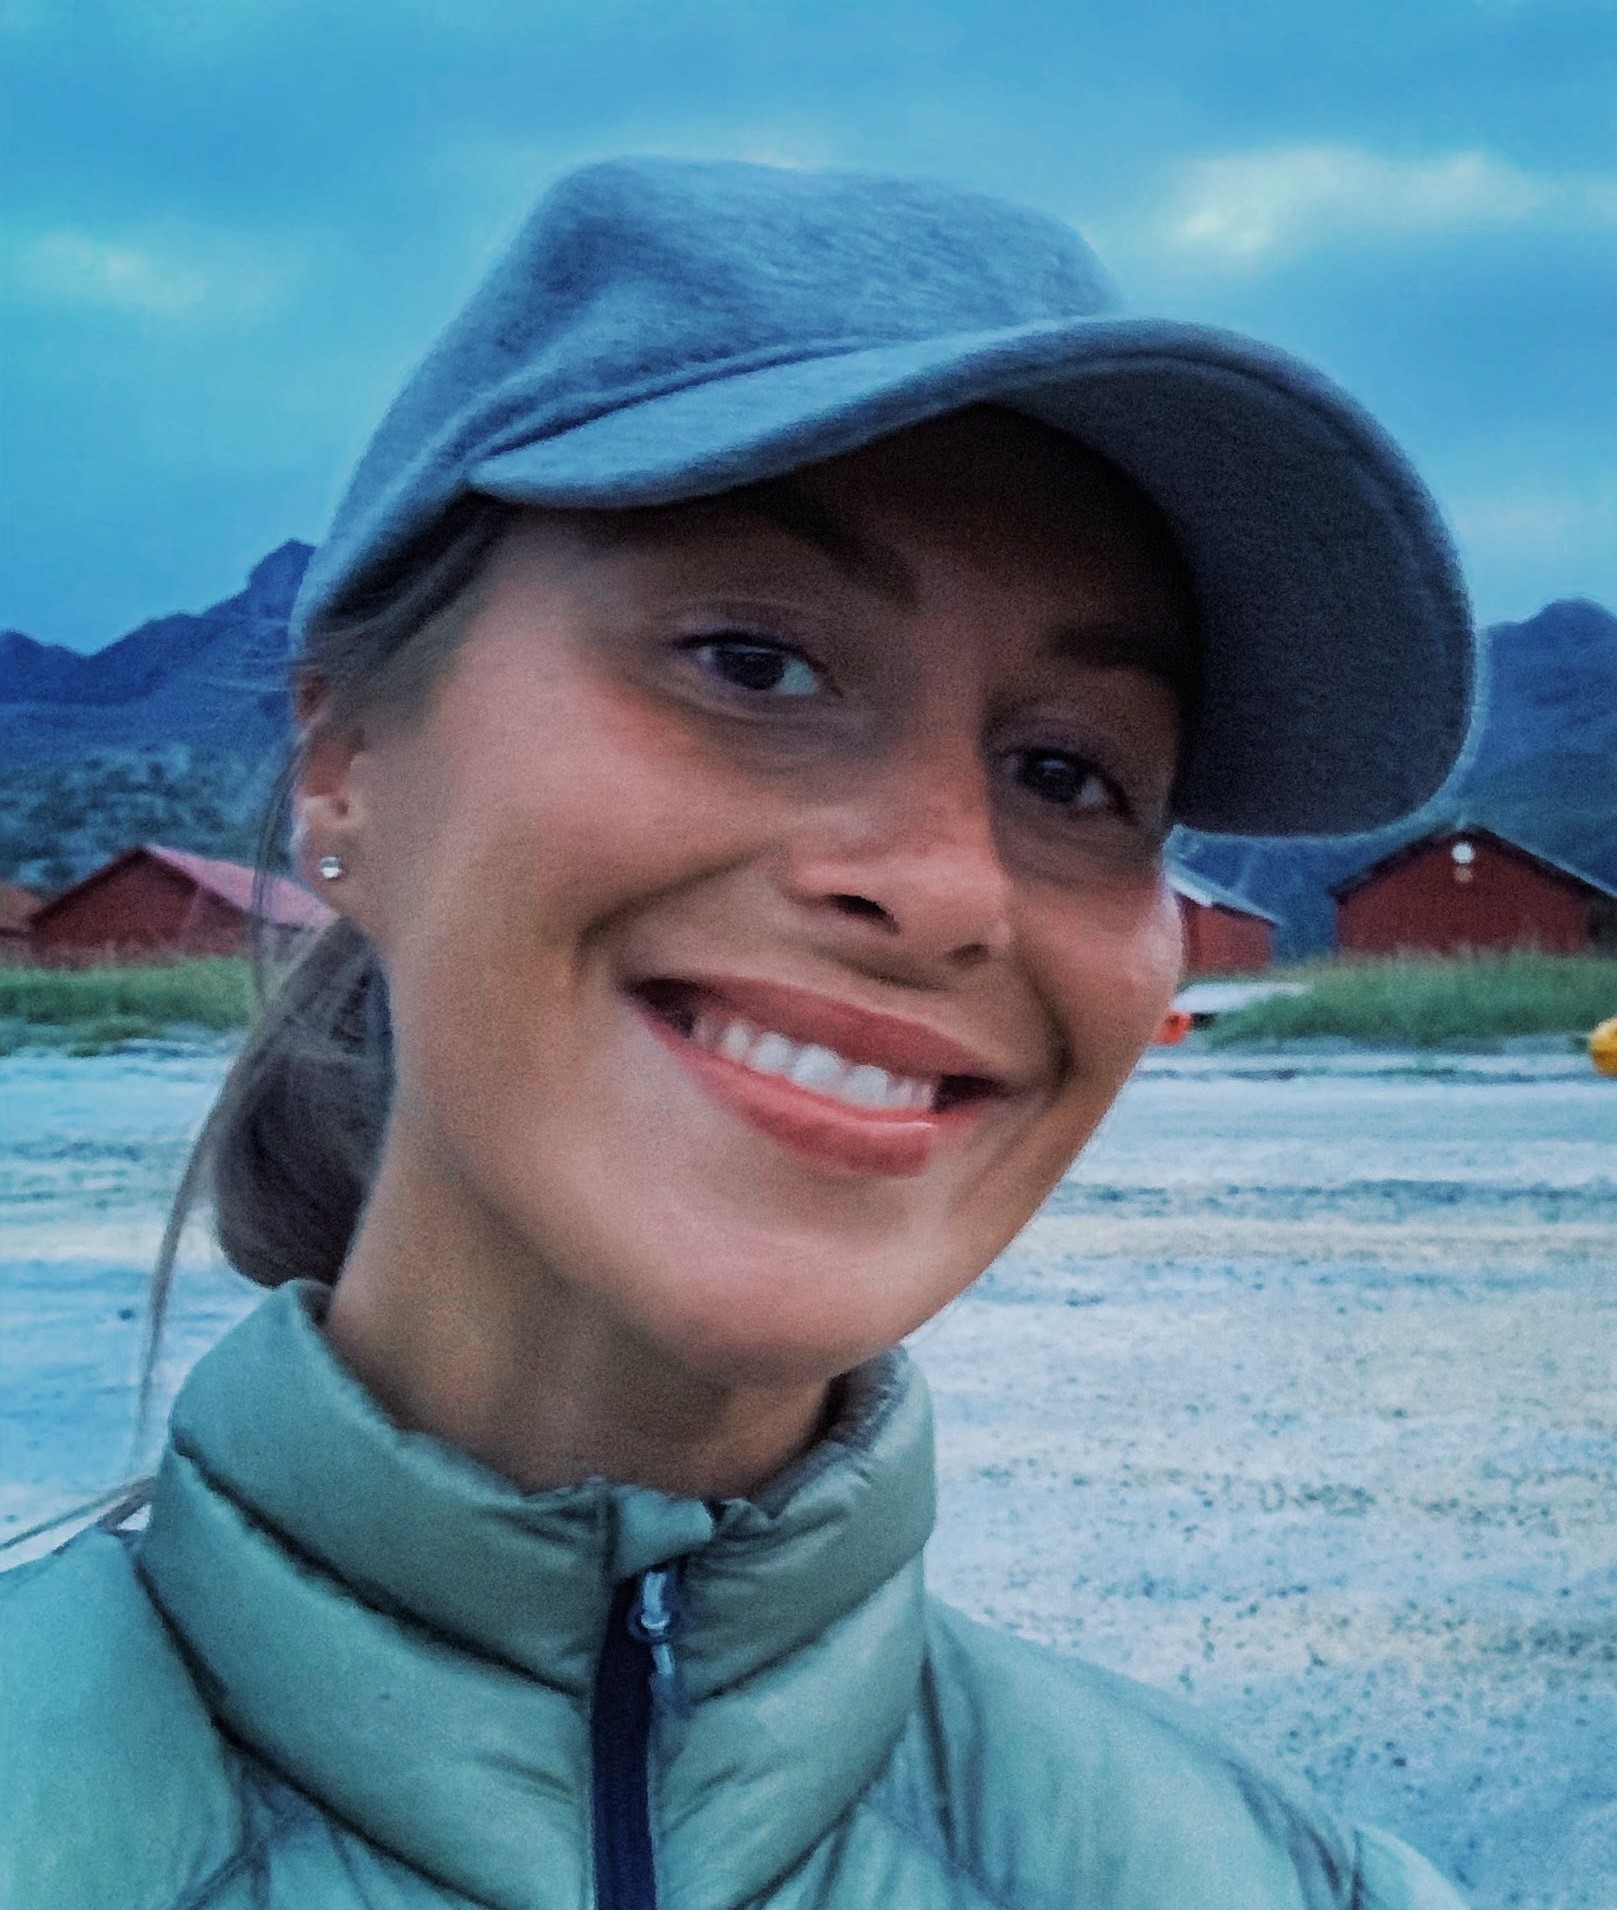
\includegraphics[height=3cm]{PROFPIC2.jpg}};
\end{tikzpicture}

\name{Karoline Barstein}

\personalinfo{
  \email{karolhb@stud.ntnu.no}
  \phone{45 86 07 15}
  \mailaddress{Stjørdalsveien 19, 7066 Trondheim}
  \printinfo{f.}{15.07.1994}

  \linkedin{linkedin.com/in/barstein}
  \github{github.com/karolhb}
}

\begin{adjustwidth}{}{-8cm}
\makecvheader
\end{adjustwidth}

\cvsection[sidebar]{Experience}

\cvevent{Junior Developer}{Systor Trondheim AS}{August 2019 - Now}{Trondheim}
\begin{itemize}
\item Work in a team with another student, and experienced fulltime employees
\item Mainly frontend development, using modern technologies like Vue and Vuetify
\item Small company - high degree of responsibility and ownership to the project
\end{itemize}

\divider

\cvevent{Summer Intern }{Kantega}{June 2019 - August 2019}{Trondheim}
\begin{itemize}
\item Worked in a multidisciplinary team with other students on a summer project for one of Kantega's clients
\item Involved in observation, ideation, user involvement and development
\item Used techniques like Google Design Sprint and Scrum, and technologies like React, Firebase and Leaflet



\end{itemize}

\divider

\cvevent{Teaching Assistant}{NTNU}{August 2018 - June 2019}{Trondheim}
\begin{itemize}
\item Courses: Physics/chemistry and Procedural and Object-Oriented Programming
\item Developed the ability to teach and explain complex problems in an intelligible way

\end{itemize}

\divider

\cvevent{Customer Care Representative}{Telia Norge}{June 2016 - June 2019}{Trondheim}
\begin{itemize}
\item Basic technical support, orders and other support
\item Developed good communication and problem solving skills

\end{itemize}

\divider

\cvevent{Wardrobe/Cover/Waiter}{The Mint}{December 2012 - April 2016}{Trondheim}


\cvsection{Key attributes}
\wheelchart{1.5cm}{0.5cm}{%
  4/8em/accent!30/Conscious of personal weaknesses, 
  6/8em/accent!40/Accurate and quality conscious,
  8/8em/accent!60/Effective learner,
  4/8em/accent!20/Resourceful
  %
}

\cvsection{References}
Provided on request.

\end{document}
